% Options for packages loaded elsewhere
% Options for packages loaded elsewhere
\PassOptionsToPackage{unicode}{hyperref}
\PassOptionsToPackage{hyphens}{url}
%
\documentclass[
  english,
  russian,
  12pt,
  a4paper,
  DIV=11,
  numbers=noendperiod]{scrreprt}
\usepackage{xcolor}
\usepackage{amsmath,amssymb}
\setcounter{secnumdepth}{5}
\usepackage{iftex}
\ifPDFTeX
  \usepackage[T1]{fontenc}
  \usepackage[utf8]{inputenc}
  \usepackage{textcomp} % provide euro and other symbols
\else % if luatex or xetex
  \usepackage{unicode-math} % this also loads fontspec
  \defaultfontfeatures{Scale=MatchLowercase}
  \defaultfontfeatures[\rmfamily]{Ligatures=TeX,Scale=1}
\fi
\usepackage{lmodern}
\ifPDFTeX\else
  % xetex/luatex font selection
\fi
% Use upquote if available, for straight quotes in verbatim environments
\IfFileExists{upquote.sty}{\usepackage{upquote}}{}
\IfFileExists{microtype.sty}{% use microtype if available
  \usepackage[]{microtype}
  \UseMicrotypeSet[protrusion]{basicmath} % disable protrusion for tt fonts
}{}
\usepackage{setspace}
% Make \paragraph and \subparagraph free-standing
\makeatletter
\ifx\paragraph\undefined\else
  \let\oldparagraph\paragraph
  \renewcommand{\paragraph}{
    \@ifstar
      \xxxParagraphStar
      \xxxParagraphNoStar
  }
  \newcommand{\xxxParagraphStar}[1]{\oldparagraph*{#1}\mbox{}}
  \newcommand{\xxxParagraphNoStar}[1]{\oldparagraph{#1}\mbox{}}
\fi
\ifx\subparagraph\undefined\else
  \let\oldsubparagraph\subparagraph
  \renewcommand{\subparagraph}{
    \@ifstar
      \xxxSubParagraphStar
      \xxxSubParagraphNoStar
  }
  \newcommand{\xxxSubParagraphStar}[1]{\oldsubparagraph*{#1}\mbox{}}
  \newcommand{\xxxSubParagraphNoStar}[1]{\oldsubparagraph{#1}\mbox{}}
\fi
\makeatother


\usepackage{longtable,booktabs,array}
\usepackage{calc} % for calculating minipage widths
% Correct order of tables after \paragraph or \subparagraph
\usepackage{etoolbox}
\makeatletter
\patchcmd\longtable{\par}{\if@noskipsec\mbox{}\fi\par}{}{}
\makeatother
% Allow footnotes in longtable head/foot
\IfFileExists{footnotehyper.sty}{\usepackage{footnotehyper}}{\usepackage{footnote}}
\makesavenoteenv{longtable}
\usepackage{graphicx}
\makeatletter
\newsavebox\pandoc@box
\newcommand*\pandocbounded[1]{% scales image to fit in text height/width
  \sbox\pandoc@box{#1}%
  \Gscale@div\@tempa{\textheight}{\dimexpr\ht\pandoc@box+\dp\pandoc@box\relax}%
  \Gscale@div\@tempb{\linewidth}{\wd\pandoc@box}%
  \ifdim\@tempb\p@<\@tempa\p@\let\@tempa\@tempb\fi% select the smaller of both
  \ifdim\@tempa\p@<\p@\scalebox{\@tempa}{\usebox\pandoc@box}%
  \else\usebox{\pandoc@box}%
  \fi%
}
% Set default figure placement to htbp
\def\fps@figure{htbp}
\makeatother



\ifLuaTeX
\usepackage[bidi=basic,provide=*]{babel}
\else
\usepackage[bidi=default,provide=*]{babel}
\fi
% get rid of language-specific shorthands (see #6817):
\let\LanguageShortHands\languageshorthands
\def\languageshorthands#1{}


\setlength{\emergencystretch}{3em} % prevent overfull lines

\providecommand{\tightlist}{%
  \setlength{\itemsep}{0pt}\setlength{\parskip}{0pt}}



 
\usepackage[style=gost-numeric,backend=biber,langhook=extras,autolang=other*]{biblatex}
\addbibresource{bib/cite.bib}

\usepackage[]{csquotes}

\KOMAoption{captions}{tableheading}
\usepackage{indentfirst}
\usepackage{float}
\floatplacement{figure}{H}
\usepackage[math,RM={Scale=0.94},SS={Scale=0.94},SScon={Scale=0.94},TT={Scale=MatchLowercase,FakeStretch=0.9},DefaultFeatures={Ligatures=Common}]{plex-otf}
\makeatletter
\@ifpackageloaded{caption}{}{\usepackage{caption}}
\AtBeginDocument{%
\ifdefined\contentsname
  \renewcommand*\contentsname{Содержание}
\else
  \newcommand\contentsname{Содержание}
\fi
\ifdefined\listfigurename
  \renewcommand*\listfigurename{Список иллюстраций}
\else
  \newcommand\listfigurename{Список иллюстраций}
\fi
\ifdefined\listtablename
  \renewcommand*\listtablename{Список таблиц}
\else
  \newcommand\listtablename{Список таблиц}
\fi
\ifdefined\figurename
  \renewcommand*\figurename{Рисунок}
\else
  \newcommand\figurename{Рисунок}
\fi
\ifdefined\tablename
  \renewcommand*\tablename{Таблица}
\else
  \newcommand\tablename{Таблица}
\fi
}
\@ifpackageloaded{float}{}{\usepackage{float}}
\floatstyle{ruled}
\@ifundefined{c@chapter}{\newfloat{codelisting}{h}{lop}}{\newfloat{codelisting}{h}{lop}[chapter]}
\floatname{codelisting}{Список}
\newcommand*\listoflistings{\listof{codelisting}{Листинги}}
\makeatother
\makeatletter
\makeatother
\makeatletter
\@ifpackageloaded{caption}{}{\usepackage{caption}}
\@ifpackageloaded{subcaption}{}{\usepackage{subcaption}}
\makeatother
\usepackage{bookmark}
\IfFileExists{xurl.sty}{\usepackage{xurl}}{} % add URL line breaks if available
\urlstyle{same}
\hypersetup{
  pdftitle={Лабораторная работа №2},
  pdfauthor={Емельянов Антон},
  pdflang={ru-RU},
  hidelinks,
  pdfcreator={LaTeX via pandoc}}


\title{Лабораторная работа №2}
\usepackage{etoolbox}
\makeatletter
\providecommand{\subtitle}[1]{% add subtitle to \maketitle
  \apptocmd{\@title}{\par {\large #1 \par}}{}{}
}
\makeatother
\subtitle{Первоначальная настройка git}
\author{Емельянов Антон}
\date{}
\begin{document}
\maketitle

\renewcommand*\contentsname{Содержание}
{
\setcounter{tocdepth}{1}
\tableofcontents
}
\listoffigures
\listoftables

\setstretch{1.5}
\chapter{Цель
работы}\label{ux446ux435ux43bux44c-ux440ux430ux431ux43eux442ux44b}

Изучить идеологию и применение средств контроля версий. Освоить умения
по работе с git..

\chapter{Задание}\label{ux437ux430ux434ux430ux43dux438ux435}

Здесь приводится описание задания в соответствии с рекомендациями
методического пособия и выданным вариантом.

\chapter{Теоретическое
введение}\label{ux442ux435ux43eux440ux435ux442ux438ux447ux435ux441ux43aux43eux435-ux432ux432ux435ux434ux435ux43dux438ux435}

Здесь описываются теоретические аспекты, связанные с выполнением работы.

Например, в табл.~\ref{tbl-std-dir} приведено краткое описание
стандартных каталогов Unix.

\begin{longtable}[]{@{}
  >{\raggedright\arraybackslash}p{(\linewidth - 2\tabcolsep) * \real{0.1014}}
  >{\raggedright\arraybackslash}p{(\linewidth - 2\tabcolsep) * \real{0.8986}}@{}}
\caption{Описание некоторых каталогов файловой системы GNU
Linux}\label{tbl-std-dir}\tabularnewline
\toprule\noalign{}
\begin{minipage}[b]{\linewidth}\raggedright
Имя каталога
\end{minipage} & \begin{minipage}[b]{\linewidth}\raggedright
Описание каталога
\end{minipage} \\
\midrule\noalign{}
\endfirsthead
\toprule\noalign{}
\begin{minipage}[b]{\linewidth}\raggedright
Имя каталога
\end{minipage} & \begin{minipage}[b]{\linewidth}\raggedright
Описание каталога
\end{minipage} \\
\midrule\noalign{}
\endhead
\bottomrule\noalign{}
\endlastfoot
\texttt{/} & Корневая директория, содержащая всю файловую \\
\texttt{/bin} & Основные системные утилиты, необходимые как в
однопользовательском режиме, так и при обычной работе всем
пользователям \\
\texttt{/etc} & Общесистемные конфигурационные файлы и файлы
конфигурации установленных программ \\
\texttt{/home} & Содержит домашние директории пользователей, которые, в
свою очередь, содержат персональные настройки и данные пользователя \\
\texttt{/media} & Точки монтирования для сменных носителей \\
\texttt{/root} & Домашняя директория пользователя \texttt{root} \\
\texttt{/tmp} & Временные файлы \\
\texttt{/usr} & Вторичная иерархия для данных пользователя \\
\end{longtable}

Более подробно про Unix см. в
\autocite{tanenbaum_book_modern-os_ru,robbins_book_bash_en,zarrelli_book_mastering-bash_en,newham_book_learning-bash_en}.

\chapter{Выполнение лабораторной
работы}\label{ux432ux44bux43fux43eux43bux43dux435ux43dux438ux435-ux43bux430ux431ux43eux440ux430ux442ux43eux440ux43dux43eux439-ux440ux430ux431ux43eux442ux44b}

Научиться оформлять отчёты с помощью легковесного языка разметки
Markdown. Переместимся в каталог 2 лабы Откроем файл report.qmd и начнём
исправлять его, превращая его в отчёт по лабе 2 используем make, чтобы
создать pdf и docx Затем загружаем файлы на github В ходе работы с
языком разметки markdown были получены базовые навыки редактуры и
обращения с отчётами Лабораторная работа №2 Первоначальная настройка git
Изучить идеологию и применение средств контроля версий. Освоить умения
по работе с git. Начнём установку ПО с git: (\textbf{?@fig-001})

Далее установим gh, а также внесём всю базовую информацию: имя
глобального пользователя, адрес электронной почты, настроим utf-8 в
выводе сообщений git. Зададим имя начальной ветки (master) и установим
параметры autocrlf и safecrlf

(\textbf{?@fig-002})

(\textbf{?@fig-003})

Сгенерируем ключи размера 4096 по алгоритму RSA и по алгоритму ed25519,
также сгенерируем pgp ключ, он понадобится для дальней привязки github.
Заодно не забудем зарегистрироваться на github (у меня уже была
регистрация, но в данном случае это почти ничего не меняет, так как
делаю я с новой виртуальной машины).

(\textbf{?@fig-004})

(\textbf{?@fig-005})

(\textbf{?@fig-006})

(\textbf{?@fig-007})

Теперь добавили ключ на Github, таким образом подключили систему к
Github.

(\textbf{?@fig-008})

Настроим автоматические подписи коммитов Git, заставим Git использовать
мой email для подписи коммитов.

(\textbf{?@fig-009})

Произведём авторизацию и создадим шаблон рабочего пространства, для
этого создадим папку и в ней образуем репозиторий, скопируем репозиторий
и, перейдя в каталог курса, удалим всё лишнее и создадим каталоги.

(\textbf{?@fig-010})

(\textbf{?@fig-011})

(\textbf{?@fig-012})

(\textbf{?@fig-013})

Затем отправим файлы на сервер.

(\textbf{?@fig-014})

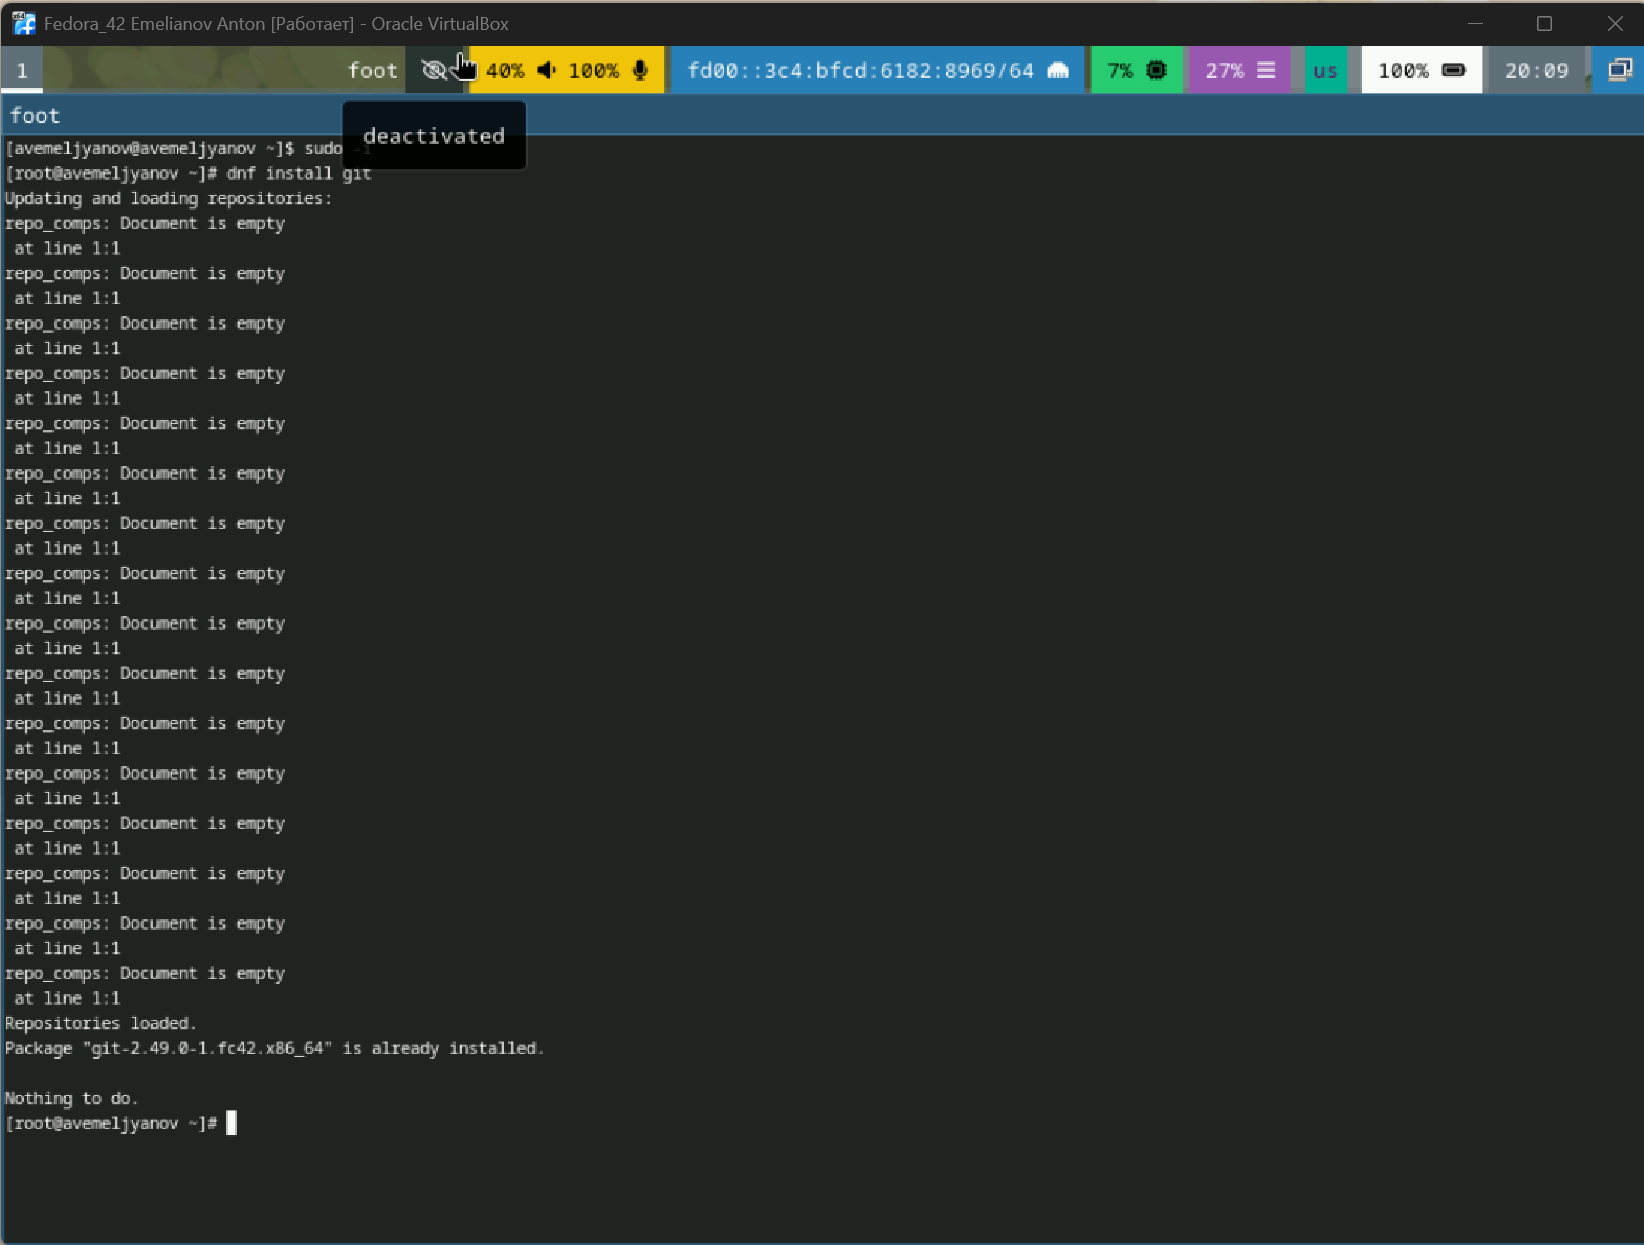
\includegraphics[width=0.7\linewidth,height=\textheight,keepaspectratio]{image/1gitinst.png}
\pandocbounded{\includegraphics[keepaspectratio]{image/2ghinst.png}}\{\#fig-001
width =70\%\}
\pandocbounded{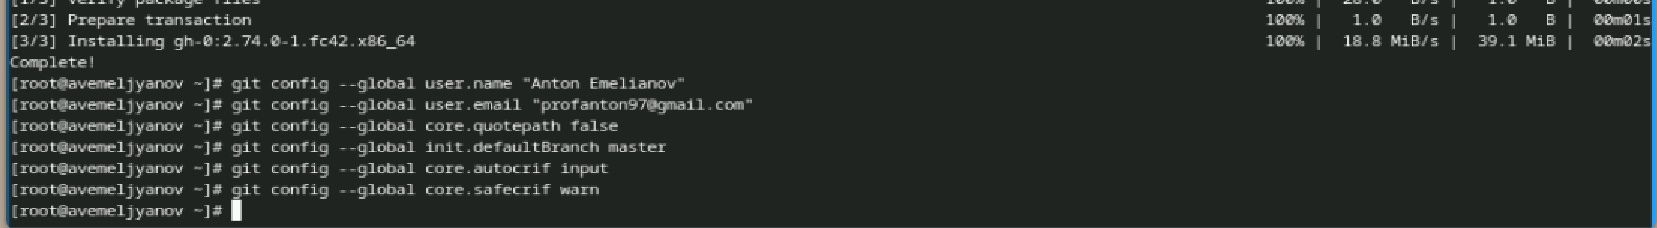
\includegraphics[keepaspectratio]{image/3basegit.png}}\{\#fig-001
width =70\%\}
\pandocbounded{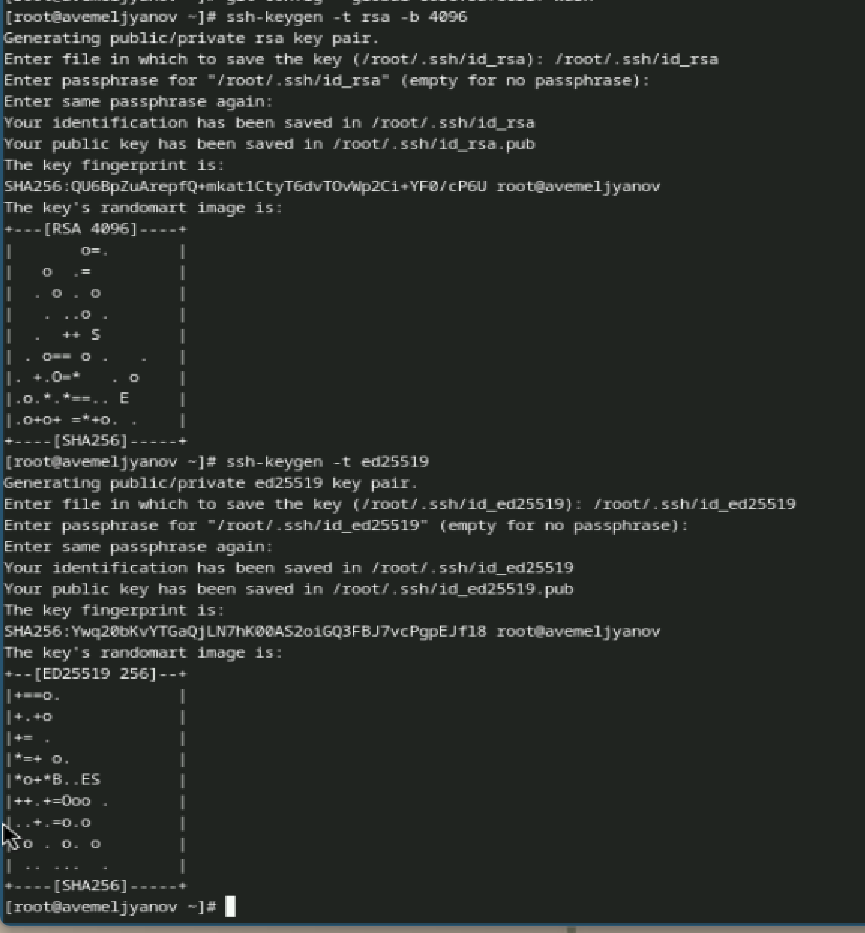
\includegraphics[keepaspectratio]{image/4sshkey.png}}\{\#fig-001
width =70\%\}
\pandocbounded{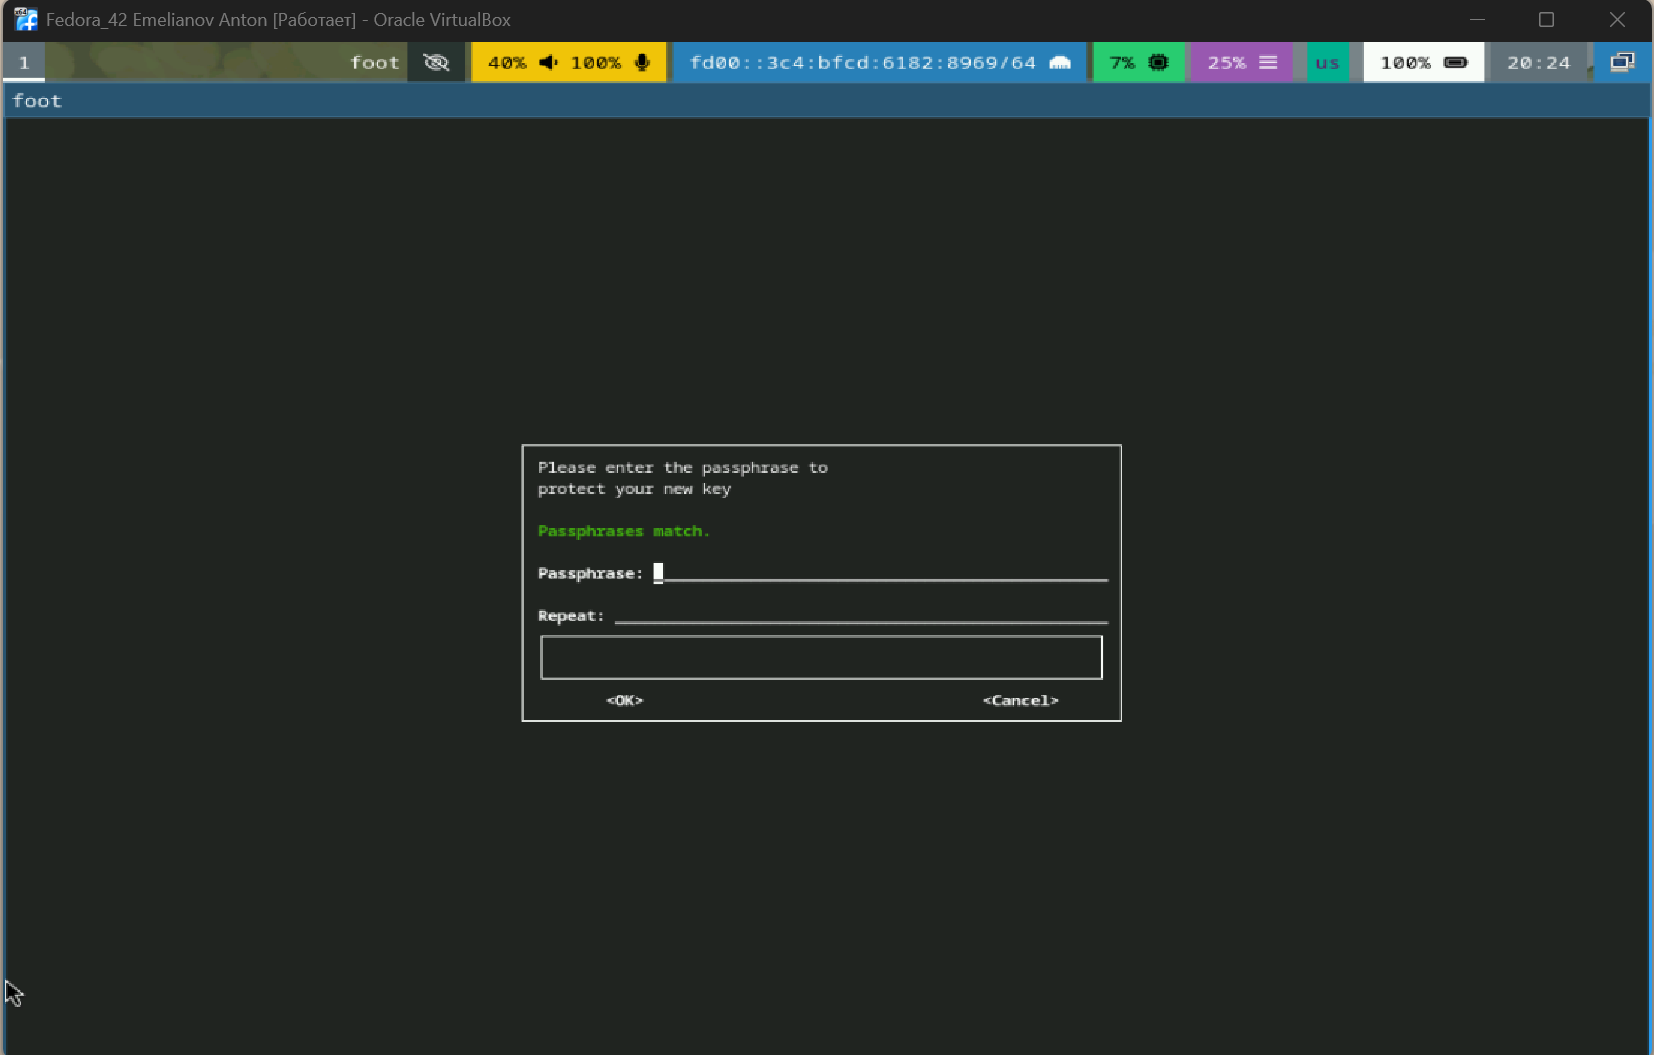
\includegraphics[keepaspectratio]{image/5pass.png}}\{\#fig-001
width =70\%\}
\pandocbounded{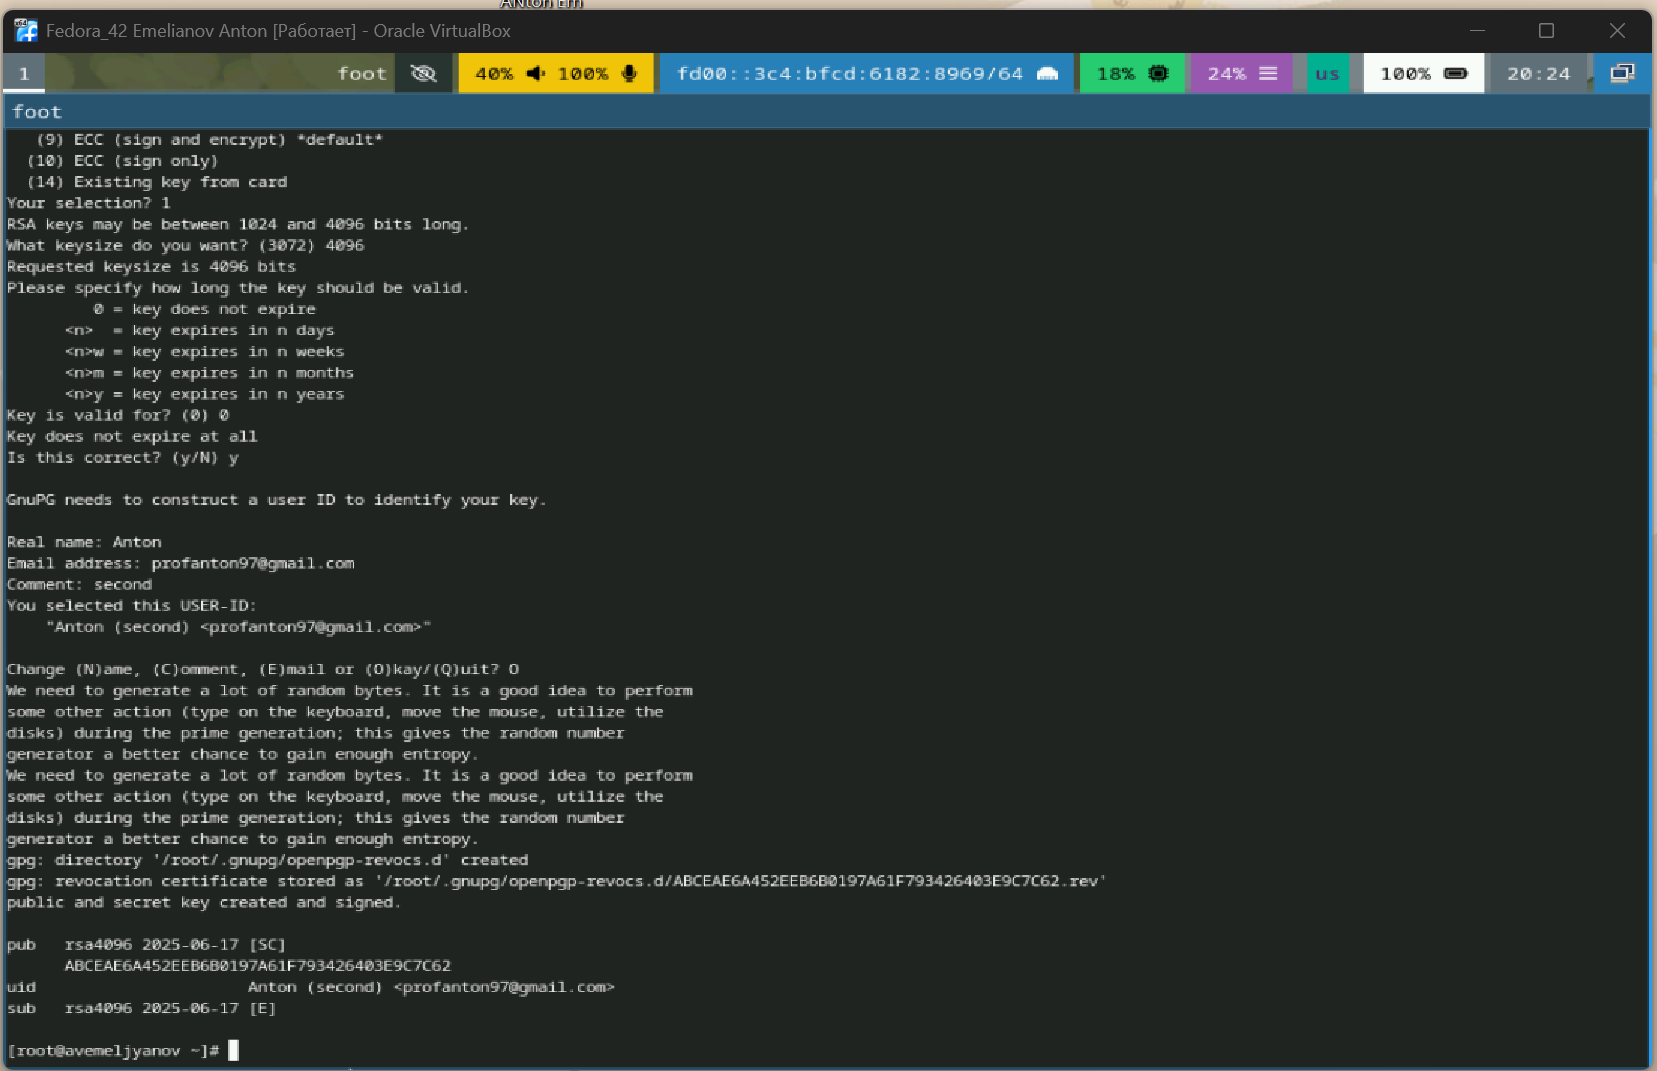
\includegraphics[keepaspectratio]{image/6keydone.png}}\{\#fig-001
width =70\%\}
\pandocbounded{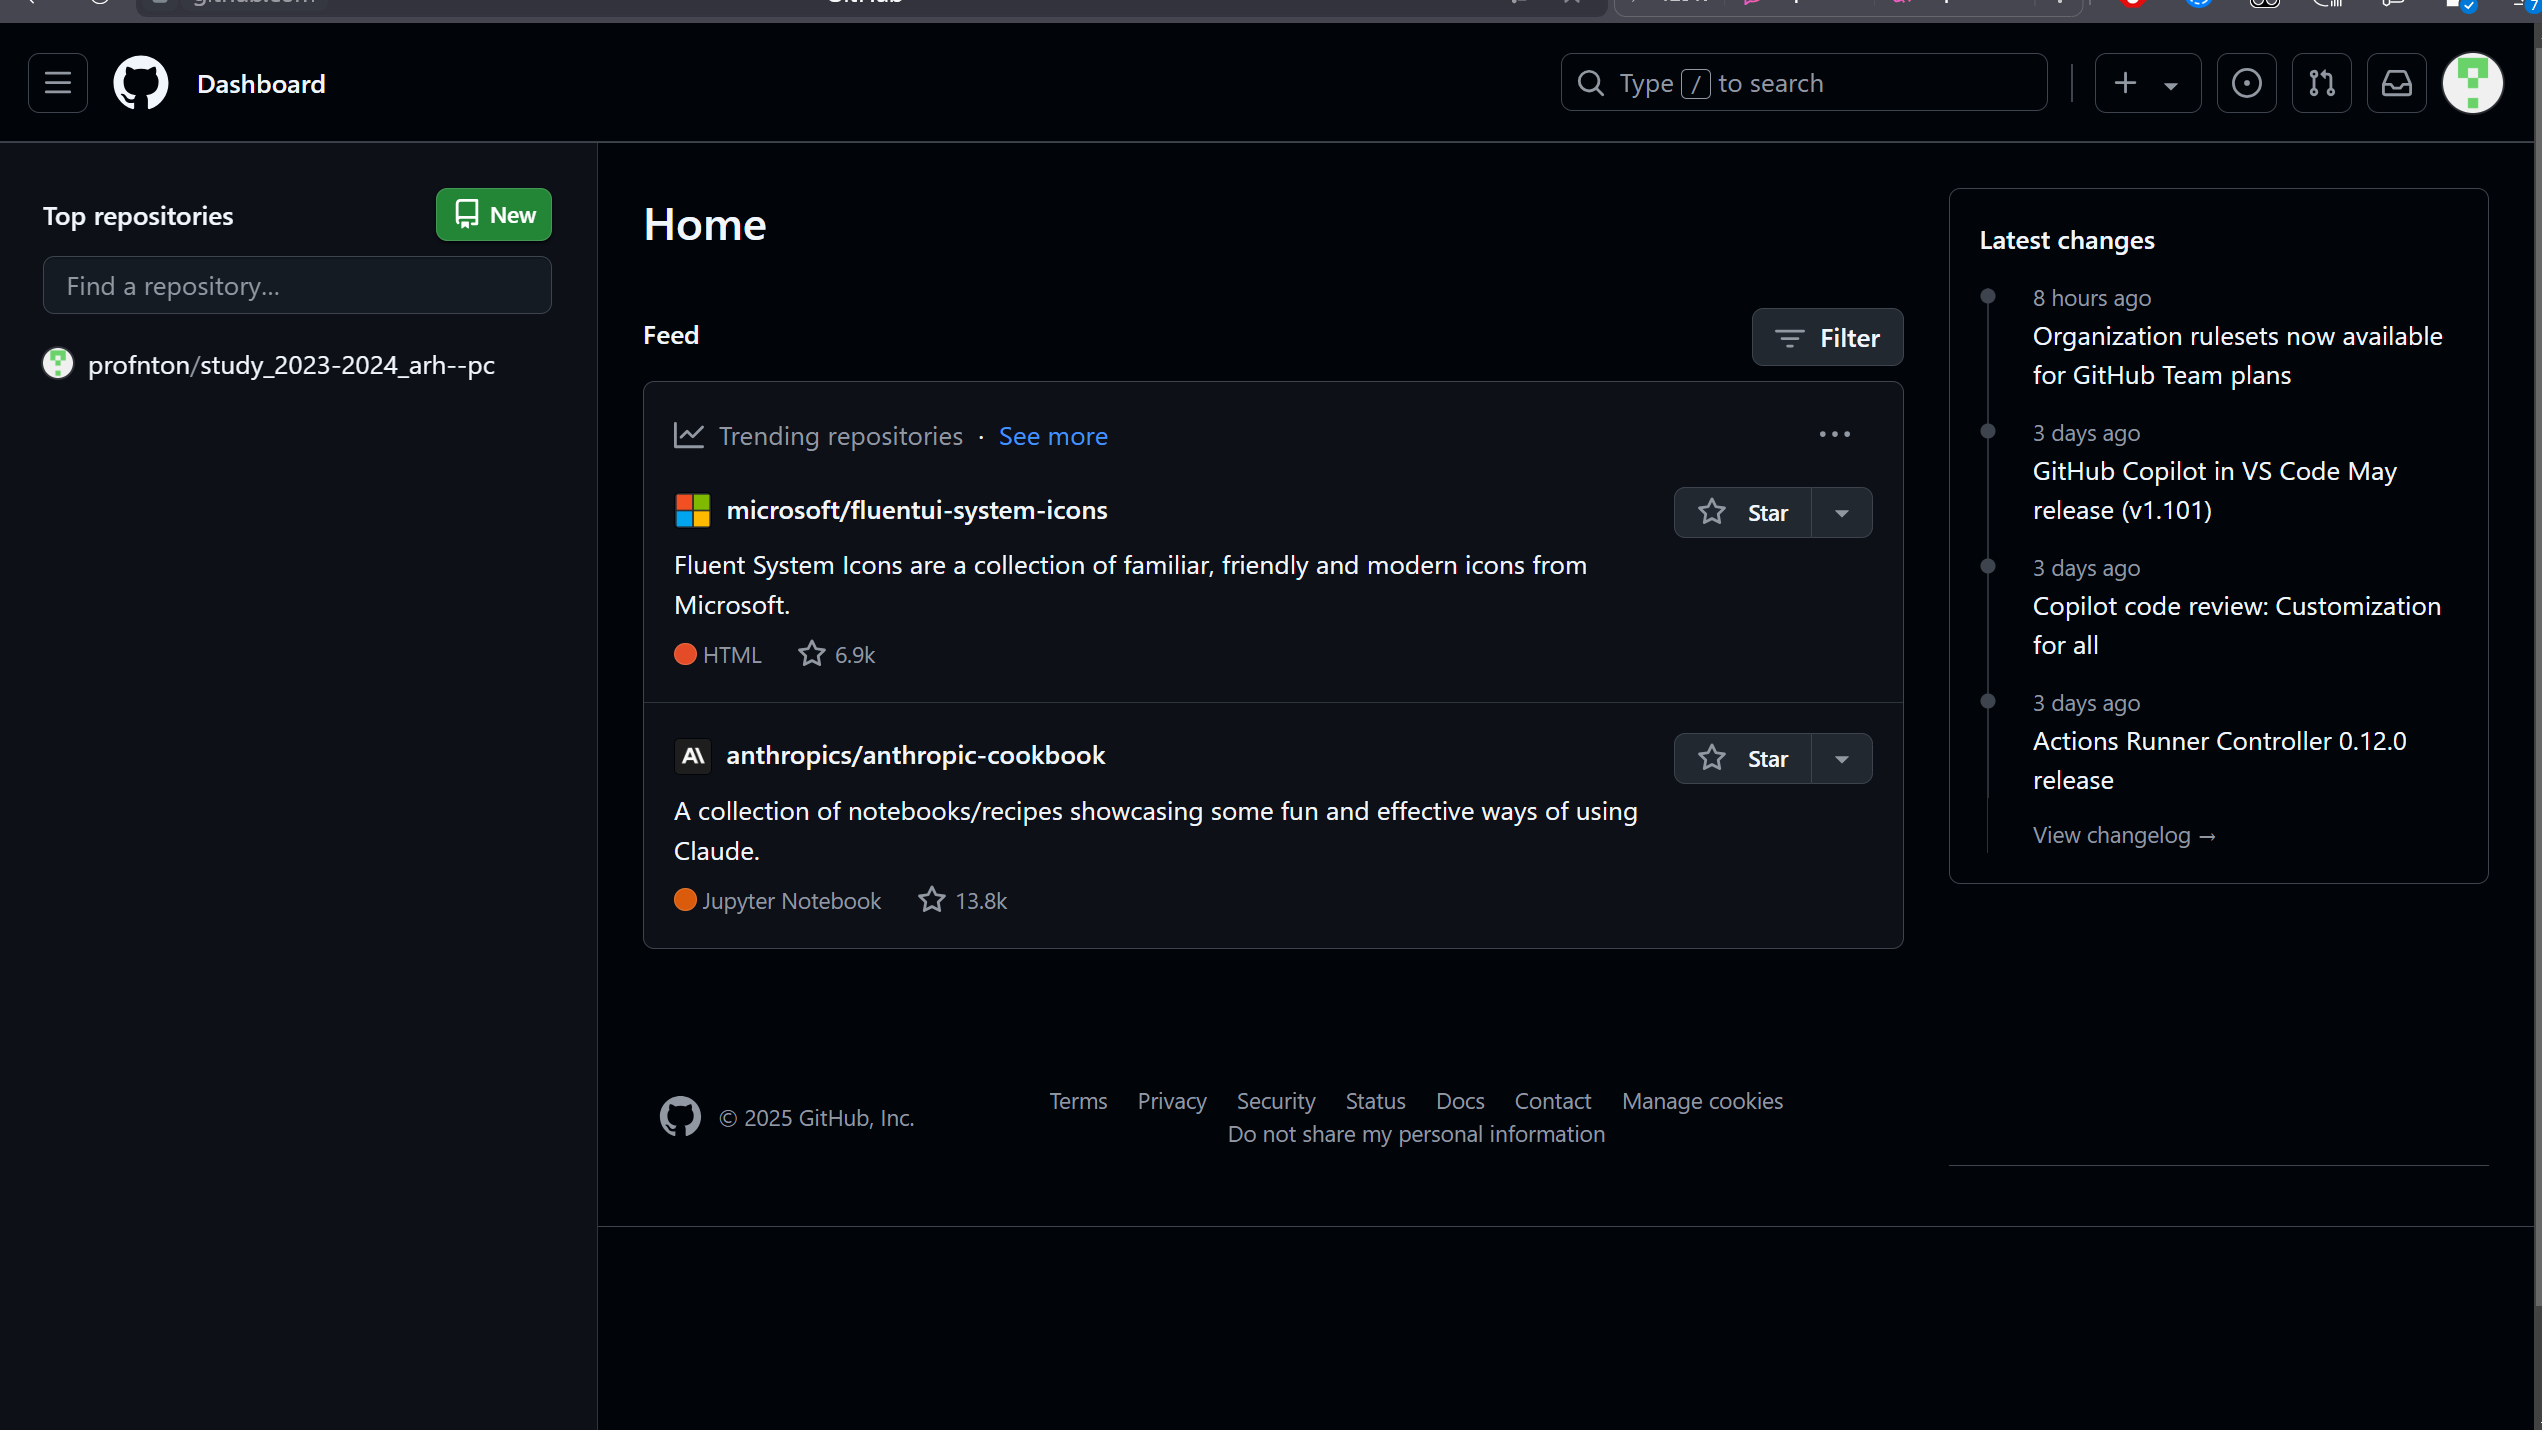
\includegraphics[keepaspectratio]{image/7githubpic.png}}\{\#fig-001
width =70\%\}
\pandocbounded{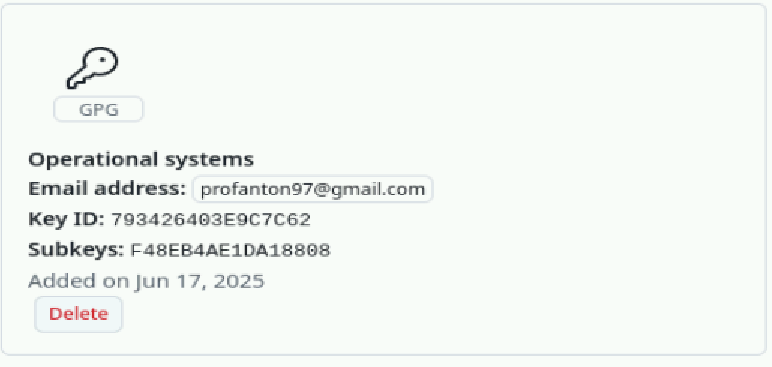
\includegraphics[keepaspectratio]{image/8githubdone.png}}\{\#fig-001
width =70\%\}
\pandocbounded{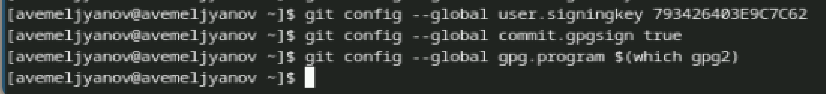
\includegraphics[keepaspectratio]{image/9sign.png}}\{\#fig-001
width =70\%\}
\pandocbounded{\includegraphics[keepaspectratio]{image/10githurray.png}}\{\#fig-001
width =70\%\}
\pandocbounded{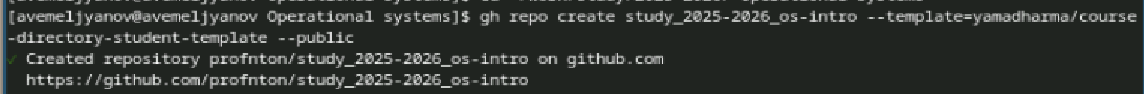
\includegraphics[keepaspectratio]{image/11ghrepo.png}}\{\#fig-001
width =70\%\}
\pandocbounded{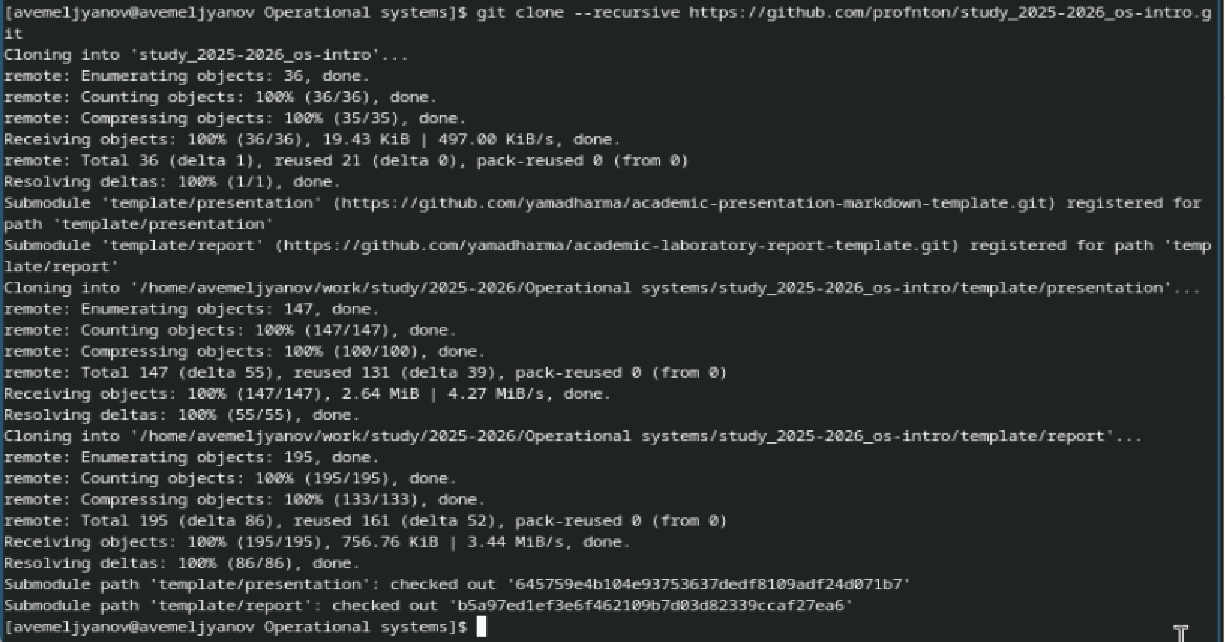
\includegraphics[keepaspectratio]{image/12gitclone.png}}\{\#fig-001
width =70\%\}
\pandocbounded{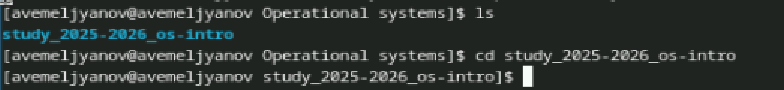
\includegraphics[keepaspectratio]{image/13cdosintro.png}}\{\#fig-001
width =70\%\}
\pandocbounded{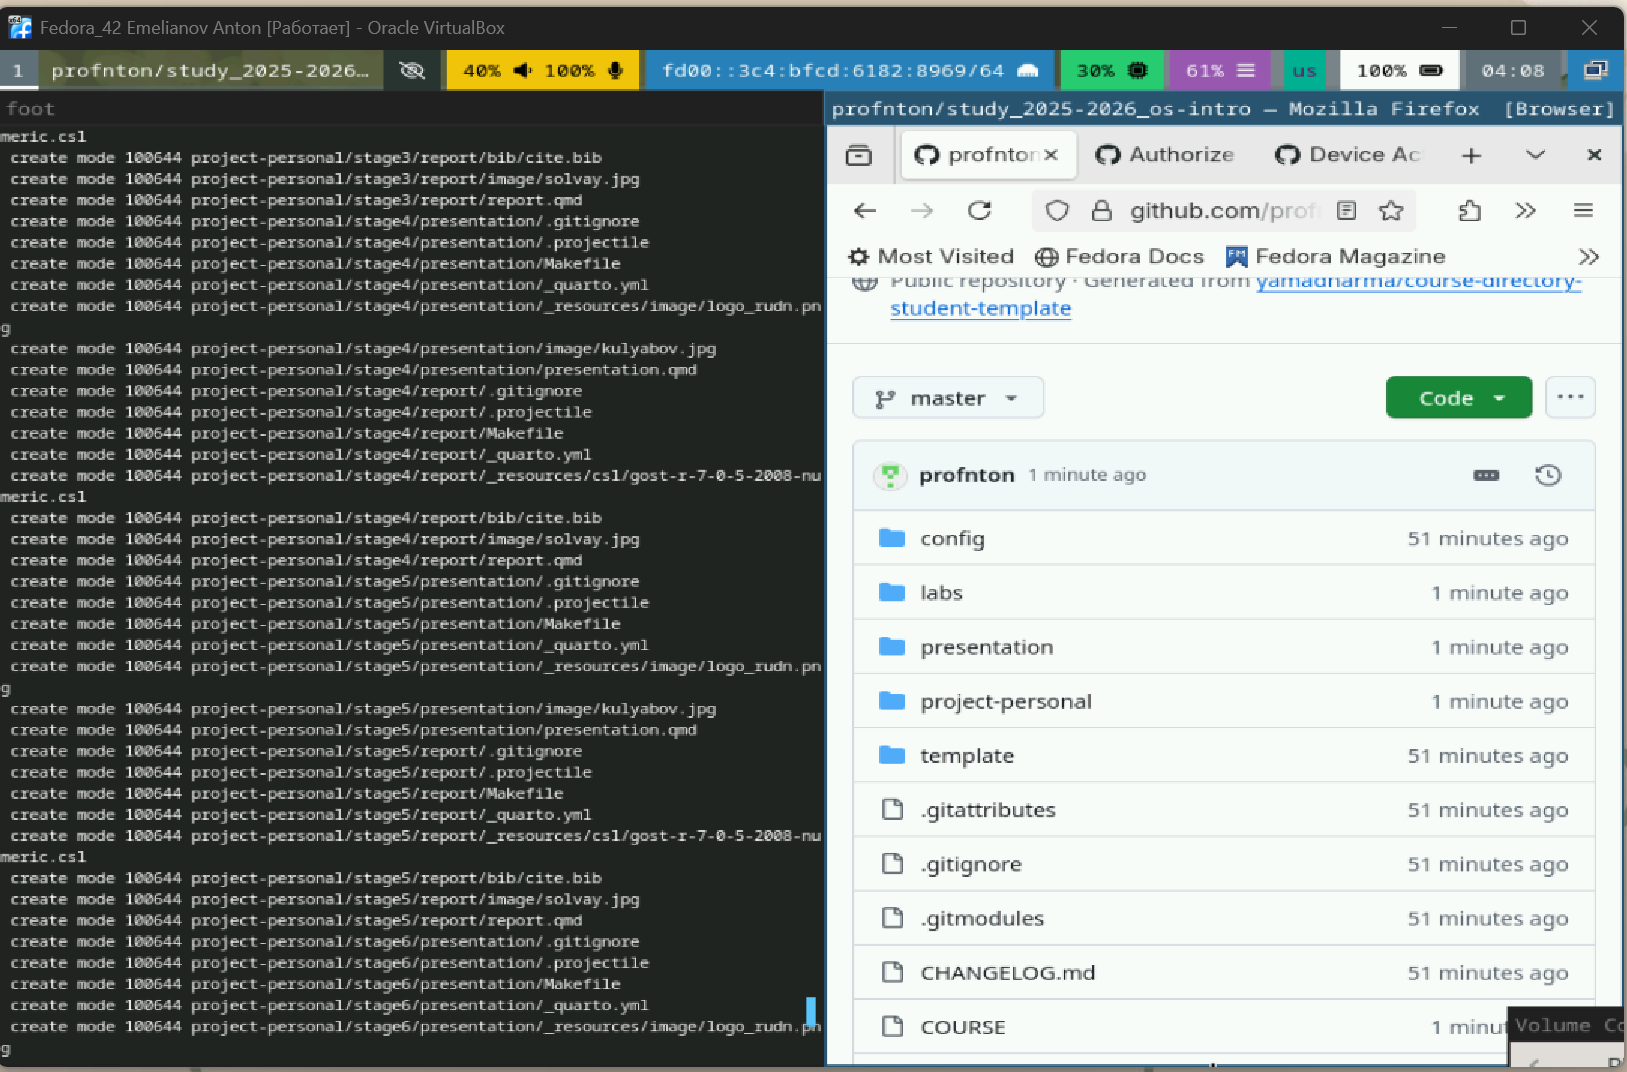
\includegraphics[keepaspectratio]{image/14pushend.png}}\{\#fig-001
width =70\%\}

\chapter{Выводы}\label{ux432ux44bux432ux43eux434ux44b}

В этой лабораторной работе мы успешно создали и настроили систему
контроля версий Git, её окружение и организовали её взаимодействие с
Github.

Что такое системы контроля версий (VCS) и для решения каких задач они
предназначаются? VCS используется для контроля изменения файлов во
времени, их основная задача - контроль версий, сравнение, возврат,
совместная работа, ветвление и резервное копирование Объясните следующие
понятия VCS и их отношения: хранилище, commit, история, рабочая копия.
Хранилище = все версии проекта, а также история их изменений Commit =
снимок состояния проекта в момент времени История = последовательность
Commit-ов

\chapter*{Список
литературы}\label{ux441ux43fux438ux441ux43eux43a-ux43bux438ux442ux435ux440ux430ux442ux443ux440ux44b}
\addcontentsline{toc}{chapter}{Список литературы}

\printbibliography[heading=none]





\end{document}
